\subsection*{Control Models}
To validate our control models, it is important to evaluate the error dynamics associated with the controllers. To do this, we begin with the comparison of the error convergence between the Adaptive Control model and the classical PD Control model. This comparison was made with a fixed, known weight, as well as no noise in the joint values.
\begin{figure}[H]
	\centering
	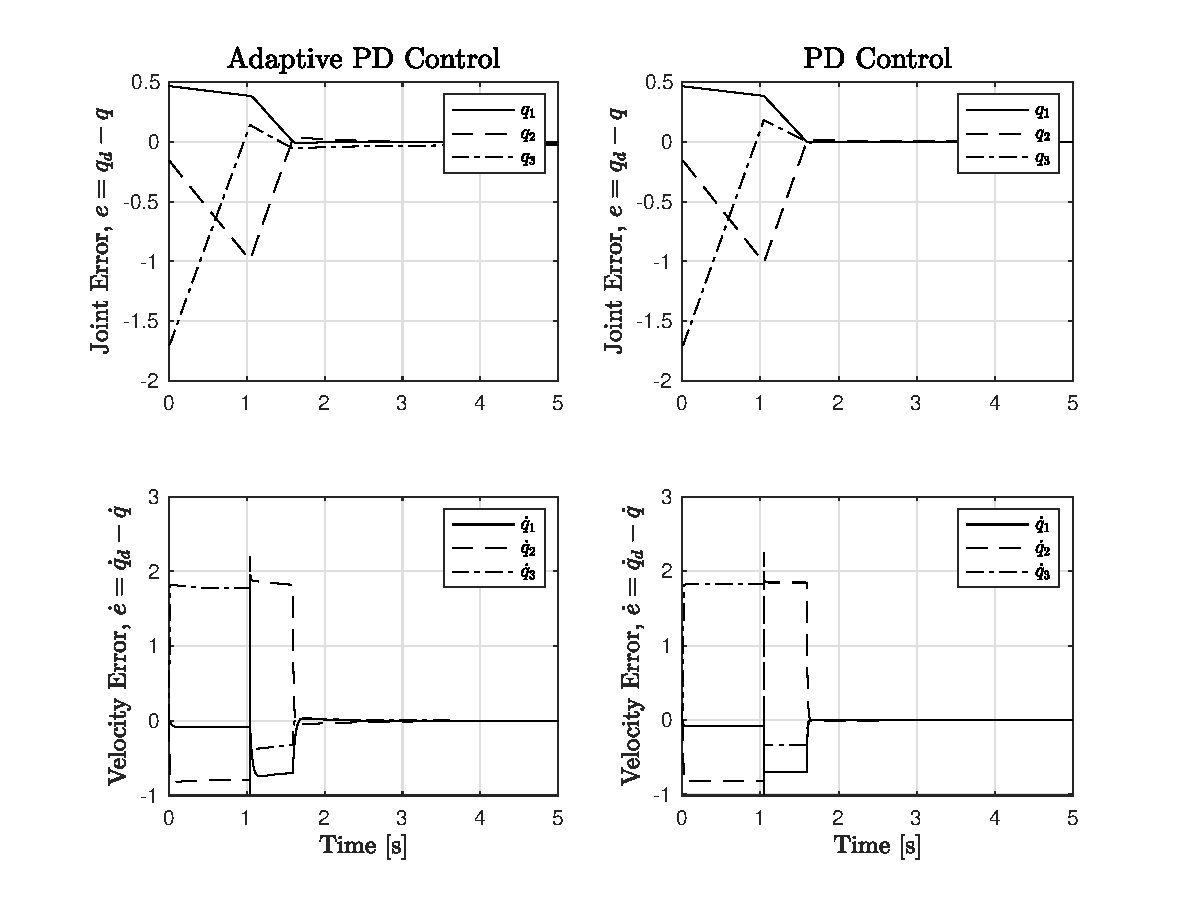
\includegraphics[width=0.7\textwidth]{figures/adpdErr.eps}
	\caption{Convergence of controller error dynamics}
	\label{fig:adpderr}
\end{figure}
As shown in Fig. \ref{fig:adpderr}, both controllers converge to the steady state value of zero in approximately the same time. One benefit to adaptive control however, is that as the mass changes (i.e. an object is picked up), the adaptation law accounts for the change in mass. With PD Control, there is no way to account for this mass addition and an increase in error is introduced.\\

We then evaluate each controller by it's ability to follow the desired trajectory provided by the $RRT^{*}$ path planning algorithm.
\begin{figure}[H]
	\centering
	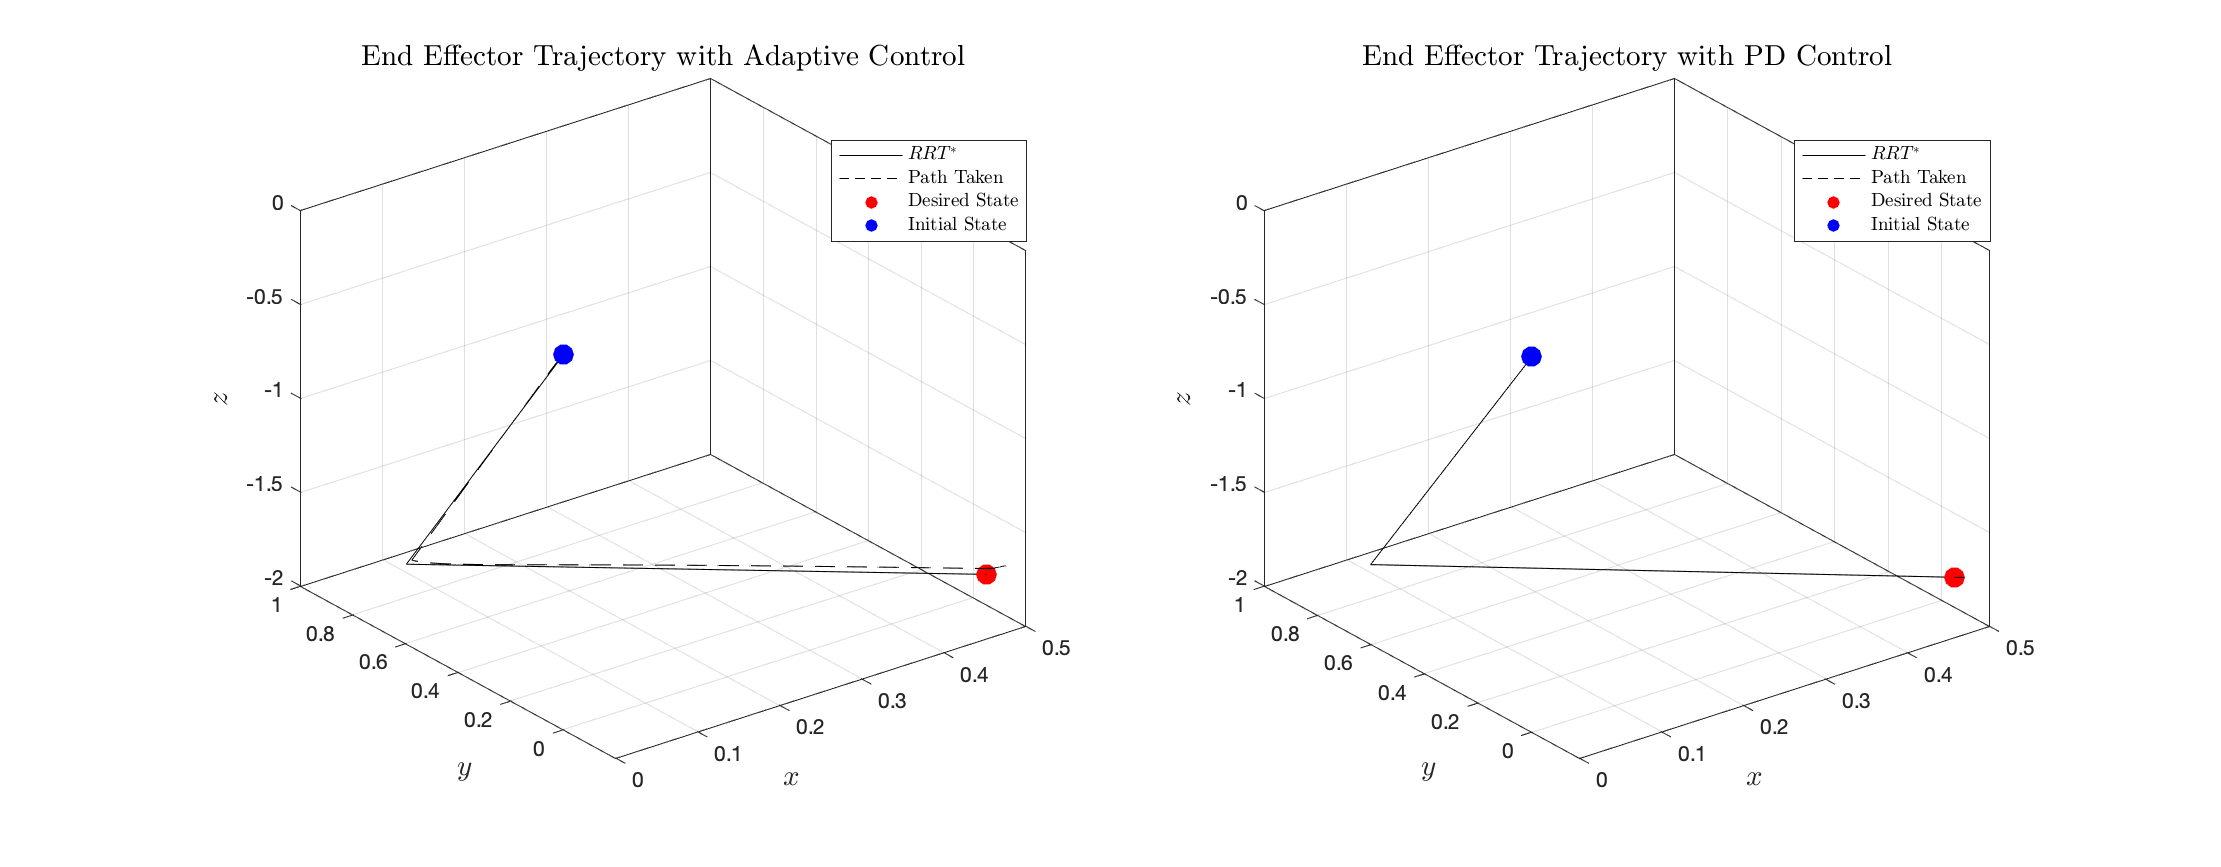
\includegraphics[width=0.9\textwidth]{figures/eeTraj.eps}
	\caption{Desired end-effector trajectory vs actual}
	\label{fig:eetraj}
\end{figure}
We can see from Fig. \ref{fig:eetraj} that in this case, the PD Controller maintains the desired trajectory more tightly than the Adaptive Control model. However, the error between the two control models is of an isnignificant degree, thus the adaptive control model is chosen for the simulation.